\chapter{研究背景}\label{chap:background}

本章では、本研究の背景について述べる。

\section{計算資源としての人}\label{ux8a08ux7b97ux8cc7ux6e90ux3068ux3057ux3066ux306eux4eba}

コンピュータのみでは解決が困難な問題を、人間を計算資源として利用することによって解決する考え方は
ヒューマンコンピュテーション\cite{humancomputation}と呼ばれる。
コンピュータは優れた処理能力を有するが、パターン認識能力など人間のほうが得意な処理分野は多く存在する。
これらの分野において人間とコンピュータがお互いの得意な領域において力を発揮することによって、
今までは実現が困難であったような処理でも実現することが可能となった。

ヒューマンコンピュテーションの例として挙げられるシステムとして、reCAPTCHA\cite{recaptcha}が存在する。
reCAPTCHAは、人間かコンピュータを識別するためのテストとして活用されているCAPTCHA\cite{captcha}を応用し、
識別を行いながらコンピュータでは識別できなかった文字の認識を人間に実行させるシステムだ。
reCAPTCHAによって、人は自分が人間であることを証明しながら、紙の本のデジタル化に貢献している。
また、文章の校正といった作業も人間のほうが得意であるが、この校正作業をインターネットを介して
他の人間に実行させるSoylent\cite{soylent}といったソフトウェアも存在する。

インターネットを介した不特定多数の人間に仕事を依頼する仕組みはクラウドソーシング\cite{riseofcrowdsourcing}と呼ばれる。
必要なときに必要なだけの人材を安価に集めることができ、近年注目を浴びている。
クラウドソーシングにおいてもヒューマンコンピュテーションの考えが反映されており、大量の人間を計算資源とした処理が実現されている。

近年ではスマートフォンの普及によって、人間はインターネットを介していつでもあらゆる場所で、様々なシステムに接続可能となった。
これは、人間がより便利にインターネットを介して情報を得られるようになったという側面と共に、
いつでもシステム側から人間とコミュニケーションが取れるようになったということでもある。
計算資源として常時アクセス可能になりつつある人間は、今まで以上に計算資源として利用されると考えられる。

ヒューマンコンピュテーションやクラウドソーシングが広まるにつれ、人間を計算資源として捉え、活用する事例は増えている。
こういった事例から、計算資源として人間とコンピュータの差がなくなりつつあるということがわかる。
人間であろうとコンピュータであろうと、処理結果を得ることが出来れば良い。
ある処理を実現する上では、人間もコンピュータも処理を実行するための同じ資源として考えることができる。

\section{プログラムの制御領域}\label{ux30d7ux30edux30b0ux30e9ux30e0ux306eux5236ux5fa1ux9818ux57df}

世界中にある様々なコンピュータやデバイスがインターネットに繋がり、プログラムによって制御されるようになってきている。
従来のプログラムは、主に計算機上や画面の中の制御を行うことが多かったが、
近年では、Arduino\footnote{http://www.arduino.cc/}やRaspberryPi\footnote{http://www.raspberrypi.org/}等の登場によって、
誰でも簡単にセンサーやアクチュエータを扱えるようになっている。
実世界から情報を得たり、実世界を制御するためのプログラムは今では誰でも簡単に扱うことができ、
プログラムはより広い領域の制御を担うようになっている。

マーク・ワイザーが提唱したユビキタスコンピューティング\cite{weiser1991computer}は、実世界環境にコンピュータを溶けこませ、
様々な活動に活かしていくものであるが、プログラムやソフトウェアを活用して実世界をよくしていくというアイデアは古くからある。
そして、様々な研究がなされている。 また、類似の概念として、Internet of
Things(以下、IoT)\cite{iot}といった概念も提唱されている。
あらゆるモノがインターネットに繋がり、その恩恵を得るといったことだが、これもプログラムによるモノの制御であると言える。

また、建築物の構成要素をプログラマブルにする試み\cite{squama}や、プログラムによってその構成を動的に変化させるモジュールについての研究もなされている。
より高性能なロボットの登場によって、今まで人間がやっていたような領域においても、プログラムの制御が有効に働くようになるだろう。
今後プログラムによる制御は更に広がり、画面内や実世界といった領域は関係なく、
あらゆる制御をプログラムで記述するようになっていくと考えられる。

\section{あらゆる処理をプログラムで記述する}\label{ux3042ux3089ux3086ux308bux51e6ux7406ux3092ux30d7ux30edux30b0ux30e9ux30e0ux3067ux8a18ux8ff0ux3059ux308b}

前述のようにプログラムが制御出来る領域は広がっている。
プログラムによって実世界を制御することは日常的になっていくと考えられる。
また、ヒューマンコンピュテーションやクラウドソーシングの考え方が普及していくにつれ、
人間とコンピュータは計算資源として区別なく扱われるようになっていく。
画面内でも実世界でも関係なく、処理内容や環境に応じて、
人間とコンピュータを使い分けていくプログラムが実現し、実行されるようになると考えられる。
特に、実世界におけるタスクを人間に処理させるといったことが可能となり、
今までは実現できなかったような処理をプログラムとして記述できるようになる。
例えば、料理をするプログラムといったものが可能だ。
料理レシピは調理する上で必要となる処理を記述するものであり、プログラムと似ている。
人間はこのレシピを見て、実行すべき処理を読み取り、その内容に従って処理を実行する。
料理レシピをプログラムとして記述するならば、図\ref{fig:background_cooking}のようになる。

\begin{figure}[htbp]
  \begin{center}
  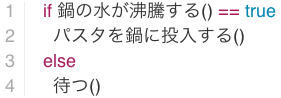
\includegraphics[width=.4\linewidth,bb=0 0 281 98]{images/background_cooking.js.png}
  \end{center}
  \caption{料理レシピをプログラム風に記述する}
  \label{fig:background_cooking}
\end{figure}

また、仕事のマニュアルなども同様である。
その時々で行うべき業務はマニュアルなどによって定義されており、人間はマニュアルを見たり、覚えておくことによって
処理を実行する。
例えば、小売店の店員の仕事は図\ref{fig:background_retail}のようなプログラムとして記述可能である。

\begin{figure}[htbp]
  \begin{center}
  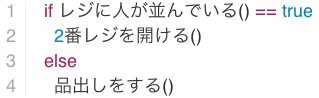
\includegraphics[width=.4\linewidth,bb=0 0 319 98]{images/background_retail.js.png}
  \end{center}
  \caption{小売店の店員の挙動をプログラム風に記述する}
  \label{fig:background_retail}
\end{figure}

レシピやマニュアルといったように、人間が実行すべき処理を記述してある手順書は多く存在する。
これは、ただ実行する対象が人間なだけであって、プログラムであると言える。
人間にとっての処理もコンピュータにとっての処理も、ほぼ同じ記法で記述することが可能だ。

このように、実世界で人間が今まで行っていたようなタスクでも、プログラムとして記述することが可能である。
また、こういったタスクであっても、人間とコンピュータが分業することによってより効率的にしたり、
人間の負担を減らすことが可能である。
そもそも、人間とコンピュータでは得意な分野や実現可能な処理が異なる。
人間は柔軟な思考能力や身体を所有することから、パターン認識や感性判断の必要な処理、実世界から情報を取得したり、干渉することが得意である。
また、意思決定も人間が実行すべき処理だ。
コンピュータは高速な演算能力を有することから、計算や記憶、正確なセンシングなどを担うべきである。
タスクをプログラムとして記述し、コンピュータでも出来ることやコンピュータのほうが得意なことに関しては
コンピュータに実行させ、人間は人間にしかできないことや人間のほうが得意なことに専念することが可能となる。

実世界のタスク等の記述も含めた、人間とコンピュータの処理を融合させたプログラムを記述することが出来れば、
コンピュータによる支援を受けたより効率的なタスク実行などが可能となり、有用である言える。
しかし、現状ではこのプログラムを実行するような環境は整っていない。
人間とコンピュータをプログラム上において同じような記法で扱える仕組みはクラウドソーシング分野での利用に限られている。
想定する利用シーンは知的活動に限られており、実世界でのタスクを処理するようなことはできない。
「料理をする」といったプログラムは、インターネットを介した人間に実行してもらっても無意味である。
また、自分の日常的な活動をプログラムで記述したいという時でも、自分自身を実行対象にすることができない。
家庭内でのタスクをプログラムしたい場合であれば、家族に実行対象を限定したい。
これらの問題から、クラウドソーシングを利用した手法は実世界のタスクを処理するためのプログラムを実行する用途には向かない。

そこで、本研究では、人間と計算機の処理を融合させることのできるプログラミング環境を提案する。
このプログラミング環境は以下のような特徴を持つ

\begin{itemize}
\itemsep1pt\parskip0pt\parsep0pt
\item
  人間と計算機への指示を類似の記法で実現
\item
  実行者を具体的に指定可能
\item
  実世界のタスクを処理することを考慮した実装
\end{itemize}

本研究で提案するプログラミング環境によって、新しいプログラミングの可能性を追求する。

\section{まとめ}\label{ux307eux3068ux3081}

本章では、プログラムの現状について示し、人間とコンピュータが対等な処理実行のリソースであるということを示した。
また、プログラムが実行対象を選ばない汎用的な処理記述フォーマットであることを示し、あらゆる処理を記述するためのプログラミング環境の実現に向けた
状況を考察した。
